\documentclass[11pt,a4paper]{article}
\usepackage{fontspec}
\usepackage{xunicode}
\usepackage{xeCJK}
\usepackage{geometry}
\geometry{left=2.5cm, right=2.5cm, top=2.5cm, bottom=2.5cm}

\usepackage{graphicx}
\usepackage{float}
\usepackage{amsmath}

\setmainfont{CMU Serif}
\setsansfont{CMU Serif}
\setmonofont{CMU Typewriter Text}

\setCJKmainfont{SimSun}
\setCJKsansfont{SimSun}
\setCJKmonofont{SimSun}

\usepackage{datetime}
\renewcommand{\today}{\number\year 年 \number\month 月 \number\day 日}
%\renewcommand{\abstractname}{}
%\renewcommand{\contentsname}{}

\title{``基于NI myDAQ的自动控制原理实验套件''设计说明}


\begin{document}
\author{自动控制原理实验室}

\maketitle

\begin{abstract}
  本项目以MATLAB/Simulink为实验环境,将National Instruments公司出品的myDAQ可编程测量设备作为模拟/数字接口,使计算机与外部硬件交互,进而设计了用于自动控制原理教学实验的三套实验设备。每个实验所需的硬件以一块板卡的形式与myDAQ连接,并可与MATLAB中的软件控制器或虚拟受控对象交互。通过更换板卡,学生可选择进行不同的实验。
\end{abstract}

\tableofcontents

\section{NI myDAQ 接线端子适配器}

\subsection{设计目的}
NI myDAQ可编程测量设备的右侧带有20个螺丝接线端子,原本被设计用于接入单根导线,可为原型实验板上的项目供电,并通过模拟数字I/O通道读取数据。在此项目中myDAQ将与固定的数个实验板卡连接,且实验板卡需要经常更换,因此需要设计一种适配器板卡,将螺丝接线端子转换为易于插拔的连接器。

\subsection{连接器选型}
考虑到设备由经验不一定丰富的学生进行操作,用于与实验板卡对接的连接器需要满足以下要求:
\begin{enumerate}
\item 连接器或线缆至少可以承载20路信号,其中包含5V/15V供电线路。
\item 具有良好的防呆(防止接反、接错位)特性;
\item 需要足够牢固,具有良好的机械性能;
\item 使用寿命足够长。
\end{enumerate}

最初考虑的是使用2.54mm间距的排针与排座进行对接。但是这种方法十分容易被连接错位,并且机械强度不够高。之后考虑了在转接器和实验板卡之间使用线缆连接。USB Type-C连接器在区分正反插的条件下可以承载20路信号,但是这种连接器和线缆成本高且不易买到。最终使用的是D-Sub 25针连接器。连接器可被焊在转接器右侧和实验板卡左侧,可以直接对接,也可以使用线缆连接。插座周围有金属外壳,可以防止接反和接错位。

\subsection{硬件设计}
转接器上除了包含必要的电源滤波、退耦电路外,设计了300mA自恢复保险丝来提供额外电气保护。myDAQ设备上只有一个蓝色指示灯,当USB设备枚举成功时会点亮。转接器上为$\pm$15V模拟组件电源、5V数字组件电源预留了指示灯。如出现电源电流过大的情况,采集卡自动关闭电源或自恢复保险丝断路,指示灯熄灭,可帮助及时发现故障。

\begin{figure}[H]\centering
  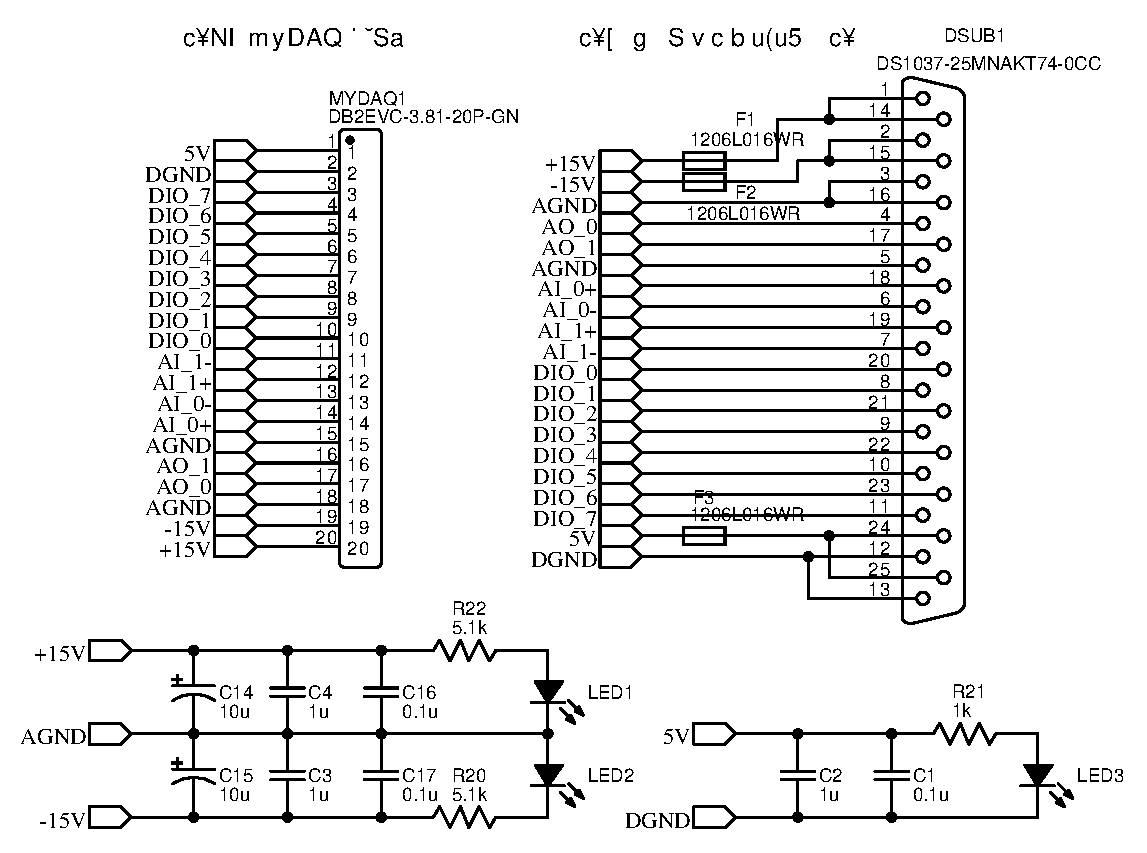
\includegraphics[width=12cm]{./figs/conv_sch.pdf}
  \caption{myDAQ接线端子适配器的原理图}\label{conv_sch}
\end{figure}


\section{模拟电路比例-积分-微分(PID)控制器}

\subsection{设计目的}
板卡上设计了基于运算放大器的PID调节器电路。myDAQ以模拟电压的形式给出一个误差量,电路将通过其比例-积分-微分环节输出一个调节量,并反馈到myDAQ的模拟输入通道中。在Simulink环境中以离散传递函数的形式建立一个虚拟对象,例如一个虚拟直流电机,并使此对象接受硬件PID调节器的控制。学生可使用拨码开关设置PID调节器的参数,使用虚拟示波器等Simulink中的工具观察PID调节器与受控对象的状态。

\subsection{PID调节器与硬件设计}
图\ref{pid_sch}为PID调节器的原理图。SW1 -- SW5为DIP拨码开关,在进行实验时,学生可选择不同参数的电阻或电容接入电路。

\begin{figure}[H]\centering
  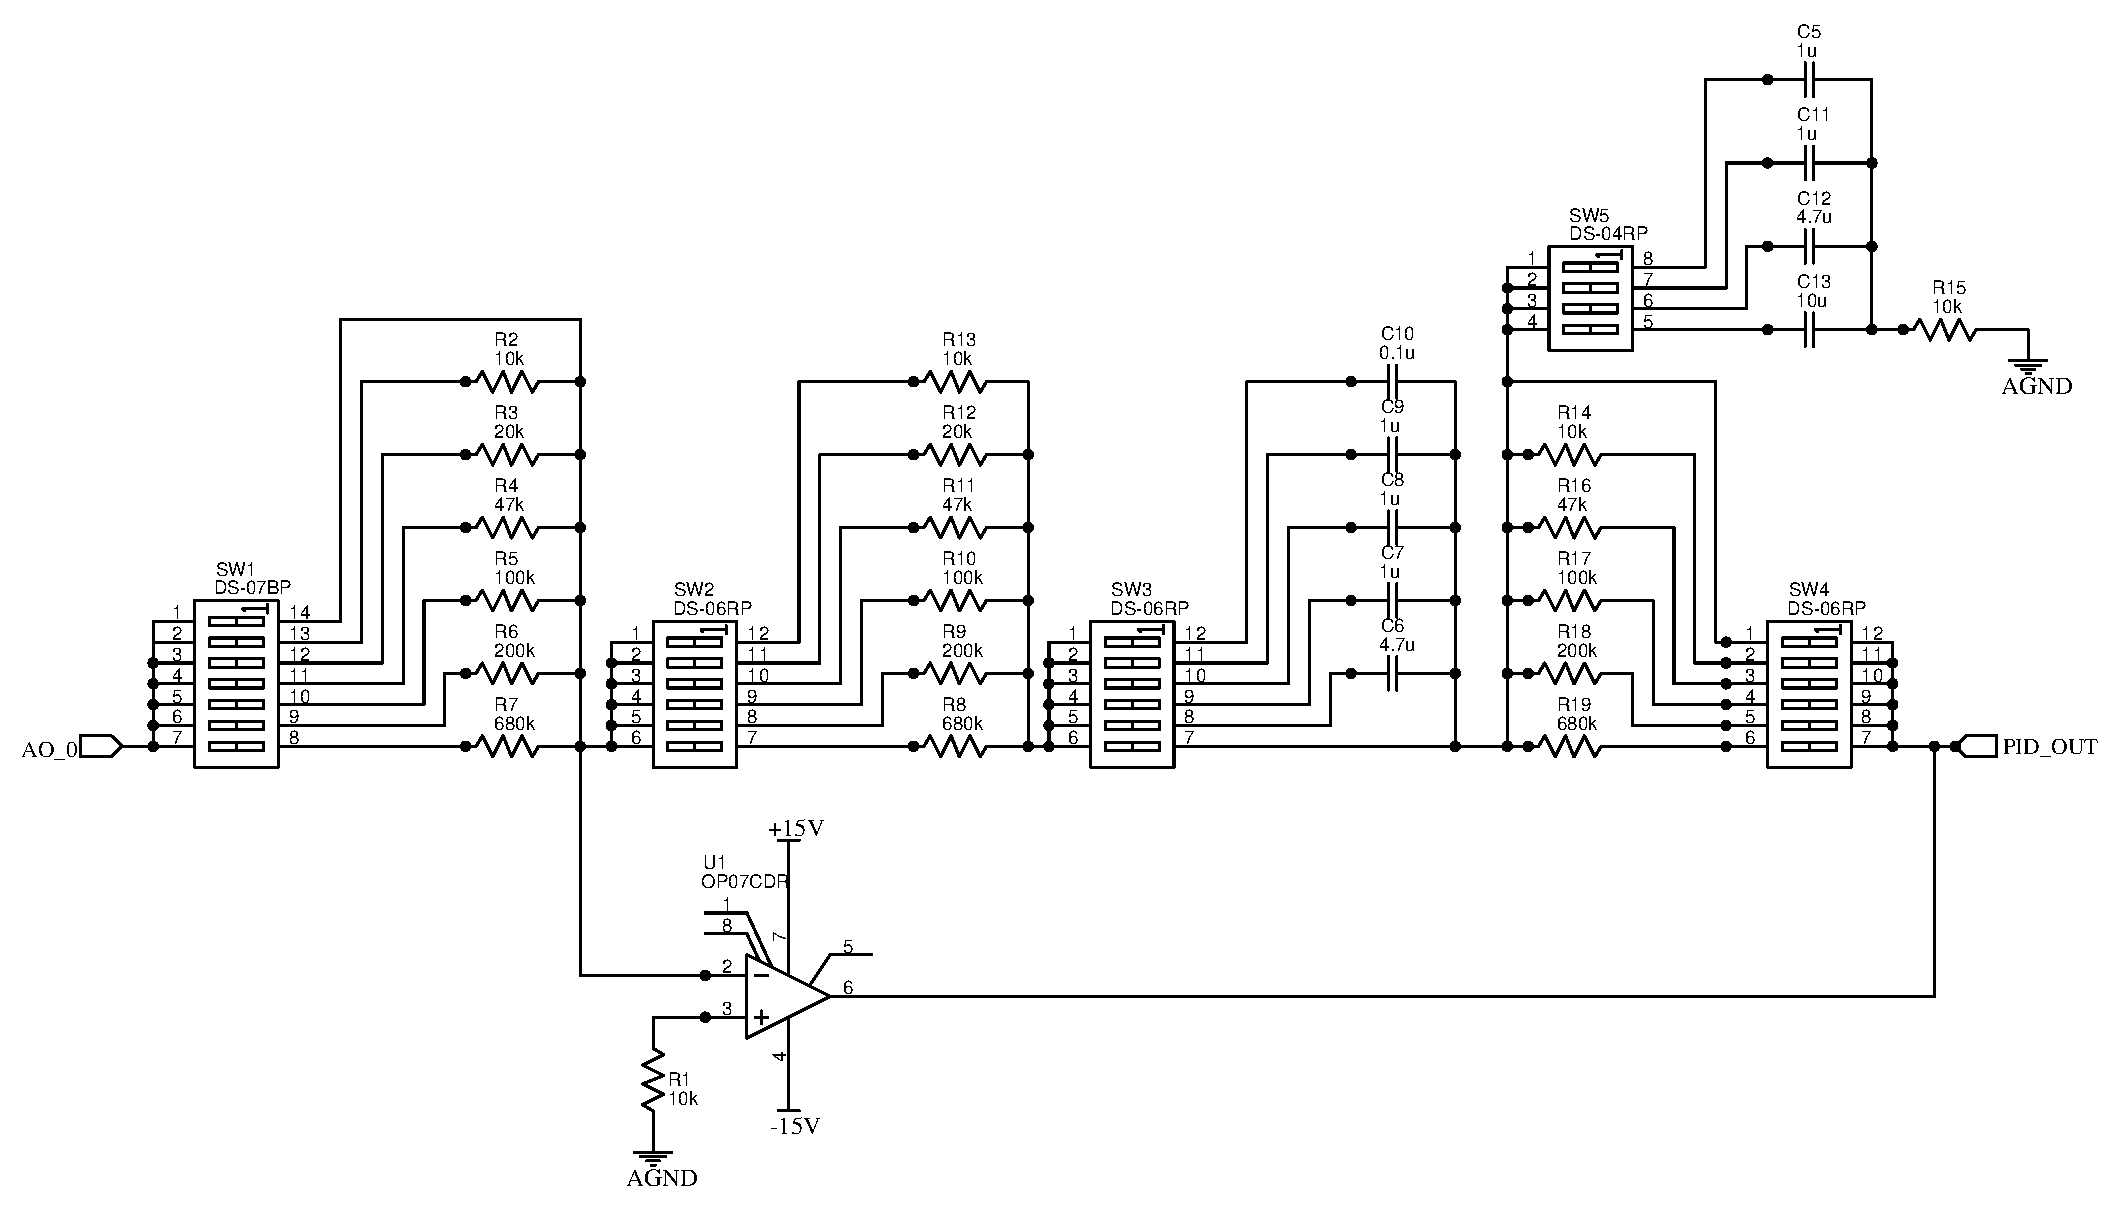
\includegraphics[width=15cm]{./figs/pid_sch.pdf}
  \caption{PID调节器的原理图}\label{pid_sch}
\end{figure}

图\ref{pid_board}为PID实验板卡的设计图。板卡上设计了原理图丝印,并将拨码开关放置于与丝印原理图匹配的位置,方便学生调节和理解。板上设计了用于供电和信号引出的焊盘,可安装2mm香蕉插座。接入外接电源后,板卡脱离myDAQ实验环境也可使用。

板上设计了调节器输出指示灯,可用于指示PID调节器正在增加或减少控制量的状态。板上有一个单圈电位器,用于手动输出-10V -- +10V模拟电压接入被控对象。PID和手动模式可使用纽子开关U7进行切换。

\begin{figure}[H]\centering
  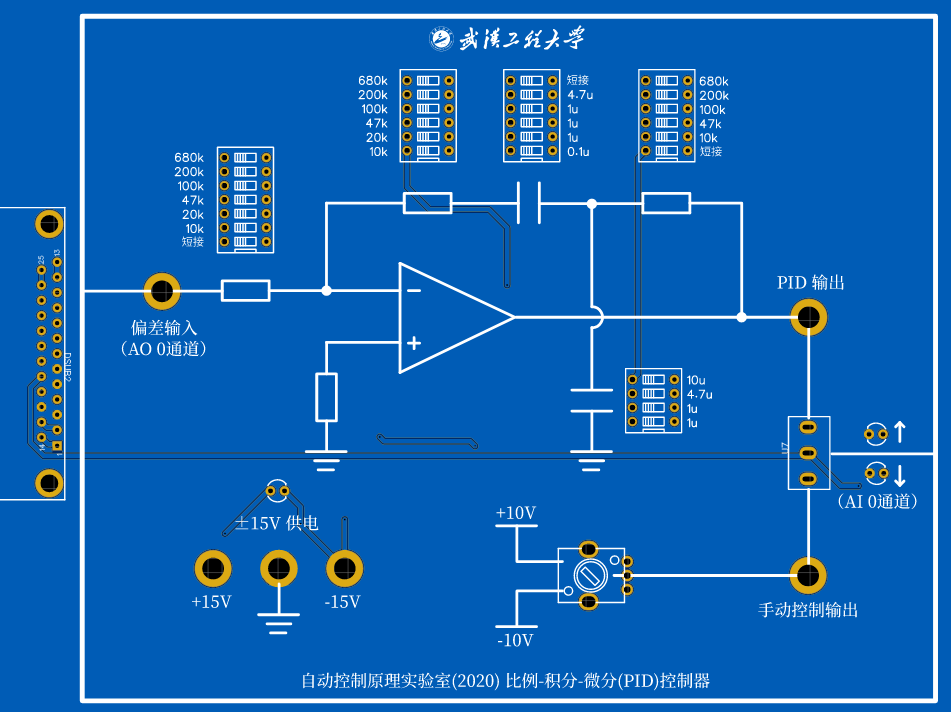
\includegraphics[width=12cm]{./figs/pid_board.png}
  \caption{PID控制器实验板卡设计图}\label{pid_board}
\end{figure}

\subsection{虚拟对象的Simulink模型}



\section{直流电机调速实验}



\section{温度控制实验}




\end{document}
